\documentclass[12pt]{article}

\pagestyle{empty}
\setlength{\topmargin}{0in}
\setlength{\headheight}{0in}
\setlength{\topsep}{0in}
\setlength{\textheight}{9in}
\setlength{\oddsidemargin}{0in}
\setlength{\evensidemargin}{0in}
\setlength{\textwidth}{6.5in}

\usepackage{palatino,graphics,amsmath,amssymb,enumitem}

\newcommand{\ds}{\displaystyle}
\newcommand{\vs}[1]{\vspace{#1in}}
\renewcommand{\vss}[1]{\vspace*{#1in}}
\newcommand{\bvec}{{\mathbf b}}
\newcommand{\cvec}{{\mathbf c}}
\newcommand{\dvec}{{\mathbf d}}
\newcommand{\evec}{{\mathbf e}}
\newcommand{\fvec}{{\mathbf f}}
\newcommand{\qvec}{{\mathbf q}}
\newcommand{\uvec}{{\mathbf u}}
\newcommand{\vvec}{{\mathbf v}}
\newcommand{\wvec}{{\mathbf w}}
\newcommand{\xvec}{{\mathbf x}}
\newcommand{\yvec}{{\mathbf y}}
\newcommand{\zvec}{{\mathbf y}}
\newcommand{\zerovec}{{\mathbf 0}}
\newcommand{\real}{{\mathbb R}}
\newcommand{\twovec}[2]{\left[\begin{array}{r}#1 \\ #2
    \end{array}\right]}
\newcommand{\ctwovec}[2]{\left[\begin{array}{c}#1 \\ #2
   \end{array}\right]}
\newcommand{\threevec}[3]{\left[\begin{array}{r}#1 \\ #2 \\ #3
  \end{array}\right]}
\newcommand{\cthreevec}[3]{\left[\begin{array}{c}#1 \\ #2 \\ #3
    \end{array}\right]}
\newcommand{\fourvec}[4]{\left[\begin{array}{r}#1 \\ #2 \\ #3 \\ #4
    \end{array}\right]}
\newcommand{\cfourvec}[4]{\left[\begin{array}{c}#1 \\ #2 \\ #3 \\ #4
    \end{array}\right]}
\newcommand{\mattwo}[4]{\left[\begin{array}{rr}#1 & #2 \\ #3 & #4 \\ \end{array}\right]}
\renewcommand{\span}[1]{\text{Span}\{#1\}}
\newcommand{\bcal}{{\cal B}}
\newcommand{\ccal}{{\cal C}}
\newcommand{\scal}{{\cal S}}
\newcommand{\wcal}{{\cal W}}
\newcommand{\ecal}{{\cal E}}
\newcommand{\coords}[2]{\left\{#1\right\}_{#2}}
\newcommand{\gray}[1]{\color{gray}{#1}}
\newcommand{\lgray}[1]{\color{lightgray}{#1}}
\newcommand{\rank}{\text{rank}}
\newcommand{\col}{\text{Col}}
\newcommand{\nul}{\text{Nul}}

\begin{document}

\noindent
{\bf Mathematics 227} \\ 
{\bf Eigenvalues and Eigenvectors}

\bigskip
\begin{enumerate}
\item  Suppose that $A$ is a $2\times2$ matrix and that $\vvec_1$ is
  an eigenvector with associated eigenvalue $\lambda_1 = -1$ and
  $\vvec_2$ is an eigenvector with associated eigenvalue
  $\lambda_2=\frac12$.  Sketch the vectors $A\xvec$ and $A^2\xvec$.

  \medskip
  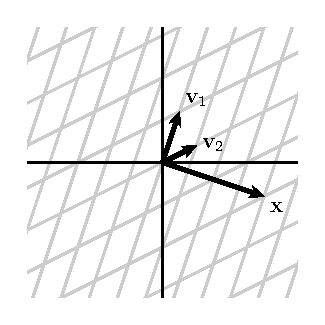
\includegraphics{26-diag.eps}

\item We have seen that the matrix
  $
  A = \left[
    \begin{array}{cc}
      1 & 2 \\
      2 & 1 \\
    \end{array}
  \right]
  $ has eigenvectors $\vvec_1=\twovec11$ and $\vvec_2=\twovec{-1}1$
  and associated eigenvalues $\lambda_1 = 3$ and $\lambda_2 = -1$.

  If $\xvec=2\vvec_1-3\vvec_2$, write $A\xvec$ as a linear combination
  of $\vvec_1$ and $\vvec_2$.

  \vs{1}
  The eigenvectors $\vvec_1$ and $\vvec_2$ form a basis $\bcal$ for
  $\real^2$.  If $\coords{\xvec}{\bcal} = \twovec{2}{-3}$, find
  $\coords{A\xvec}{\bcal}$.

  \vs{1}
  If $\coords{\xvec}{\bcal} = \twovec{c_1}{c_2}$, find
  $\coords{A\xvec}{\bcal}$.

  \vs{1}
  \newpage
  Find a matrix $D$ such that
  $\coords{A\xvec}{\bcal} = D\coords{\xvec}{\bcal}$.

  \vs{1}
  % What is the matrix $C$ such that $C\coords{\xvec}{\bcal} = \xvec$?

  % \vs{1}
  % What is the matrix $P$ such that $P\xvec = \coords{\xvec}{\bcal}$?

  % \vs{1}
  

\item
  Consider the matrix
  $A =
  \left[
    \begin{array}{ccc}
      5 & -4 & 6 \\
      -1 & 3 & -1 \\
      -2 & 3 & -3 \\
    \end{array}
  \right]
  $.
  Use Sage to find the eigenvectors using the command {\tt
    A.eigenvalues()}.

  \vs{1}
  For each eigenvector $\lambda$, find a basis for the eigenspace
  $E_\lambda$.  State the dimension of each eigenspace.

  \vs{3}
  Can you form a basis for $\real^3$ consisting of eigenvectors of
  $A$?  If so, give such a basis.

  \vs{1}
  \newpage
  Write the vector $\xvec_0 = \threevec552$ as a linear combination of
  eigenvectors.

  \vs{1.5}
  Suppose that $x_1=A\xvec_0$ and $x_2=A\xvec_1$ and so forth.
  Express $\xvec_1$, $\xvec_2$, and $\xvec_3$ as a linear combination
  of eigenvectors of $A$.

  \vs{1}
  Suppose that $\bcal$ is the basis of $\real^3$ consisting of
  eigenvectors that you found above.  Find $\coords{\xvec}{\bcal}$,
  the $\bcal$-coordinate representation of $\xvec=\threevec552$.

  \vs{1}
  Find $\coords{A\xvec}{\bcal}$.

  \vs{1}
  Find $\coords{A^2\xvec}{\bcal}$.

  \vs{1}
  Find $\coords{A^k\xvec}{\bcal}$.

  \vs{1}
  Suppose that $\xvec$ is a vector such that
  $\coords{\xvec}{\bcal} = \threevec{c_1}{c_2}{c_3}$.  What is
  $\coords{A\xvec}{\bcal}$?

  \vs{1}
  Find a matrix $D$ such that
  $D\coords{\xvec}{\bcal}=\coords{A\xvec}{\bcal}$.  
  
  \vs{1}

\end{enumerate}
\end{document}

\item Consider the matrix
  $
  A=\left[
    \begin{array}{cc}
      -1 & 2 \\
      0 & -1 \\
    \end{array}
  \right].
  $
  Find the eigenvectors $\lambda$ and a basis for the eigenspace
  $E_\lambda$.

  \vs{2}
\item Consider the matrix
  $
  A=\left[
    \begin{array}{cc}
      -1 & 0 \\
      0 & -1 \\
    \end{array}
  \right].
  $
  Find the eigenvectors $\lambda$ and a basis for the eigenspace
  $E_\lambda$.

  \vs{2}

\item  Suppose that $\lambda = 0$ is an eigenvalue of the matrix $A$.
  Remembering the definition $A\vvec=\lambda\vvec$, explain why $A$ is
  not invertible. 
  
  
  
  

\end{enumerate}


\end{document}
